\subsubsection{Página de projeto}

É na página de projeto que um docente pode consultar todas as informações sobre um projeto de uma unidade curricular da qual faz parte.

Como foi descrito na secção ~\ref{ssub:student_project}, um projeto é uma das principais entidades do sistema e como tal teve-se o cuidado em garantir que o docente encontre a informação que necessita de uma forma simples e eficiente.

A diferença entre o conteúdo disponível entre a página de um projeto de um docente e de um aluno, são:

\begin{itemize}
	\item Edição de conteúdo do projeto sem necessidade de ser redirecionado para outra página
	\item Visualização e acesso as entregas efetuadas pelos alunos inscritos na unidade curricular em que o projeto de insere
	\item Ações de publicação e encerramento de um projeto
\end{itemize}

Na Figura~\ref{fig:teacher_project} pode ser consultada uma imagem demonstrativa da página desenvolvida.

\begin{figure}[H]
  \centering
  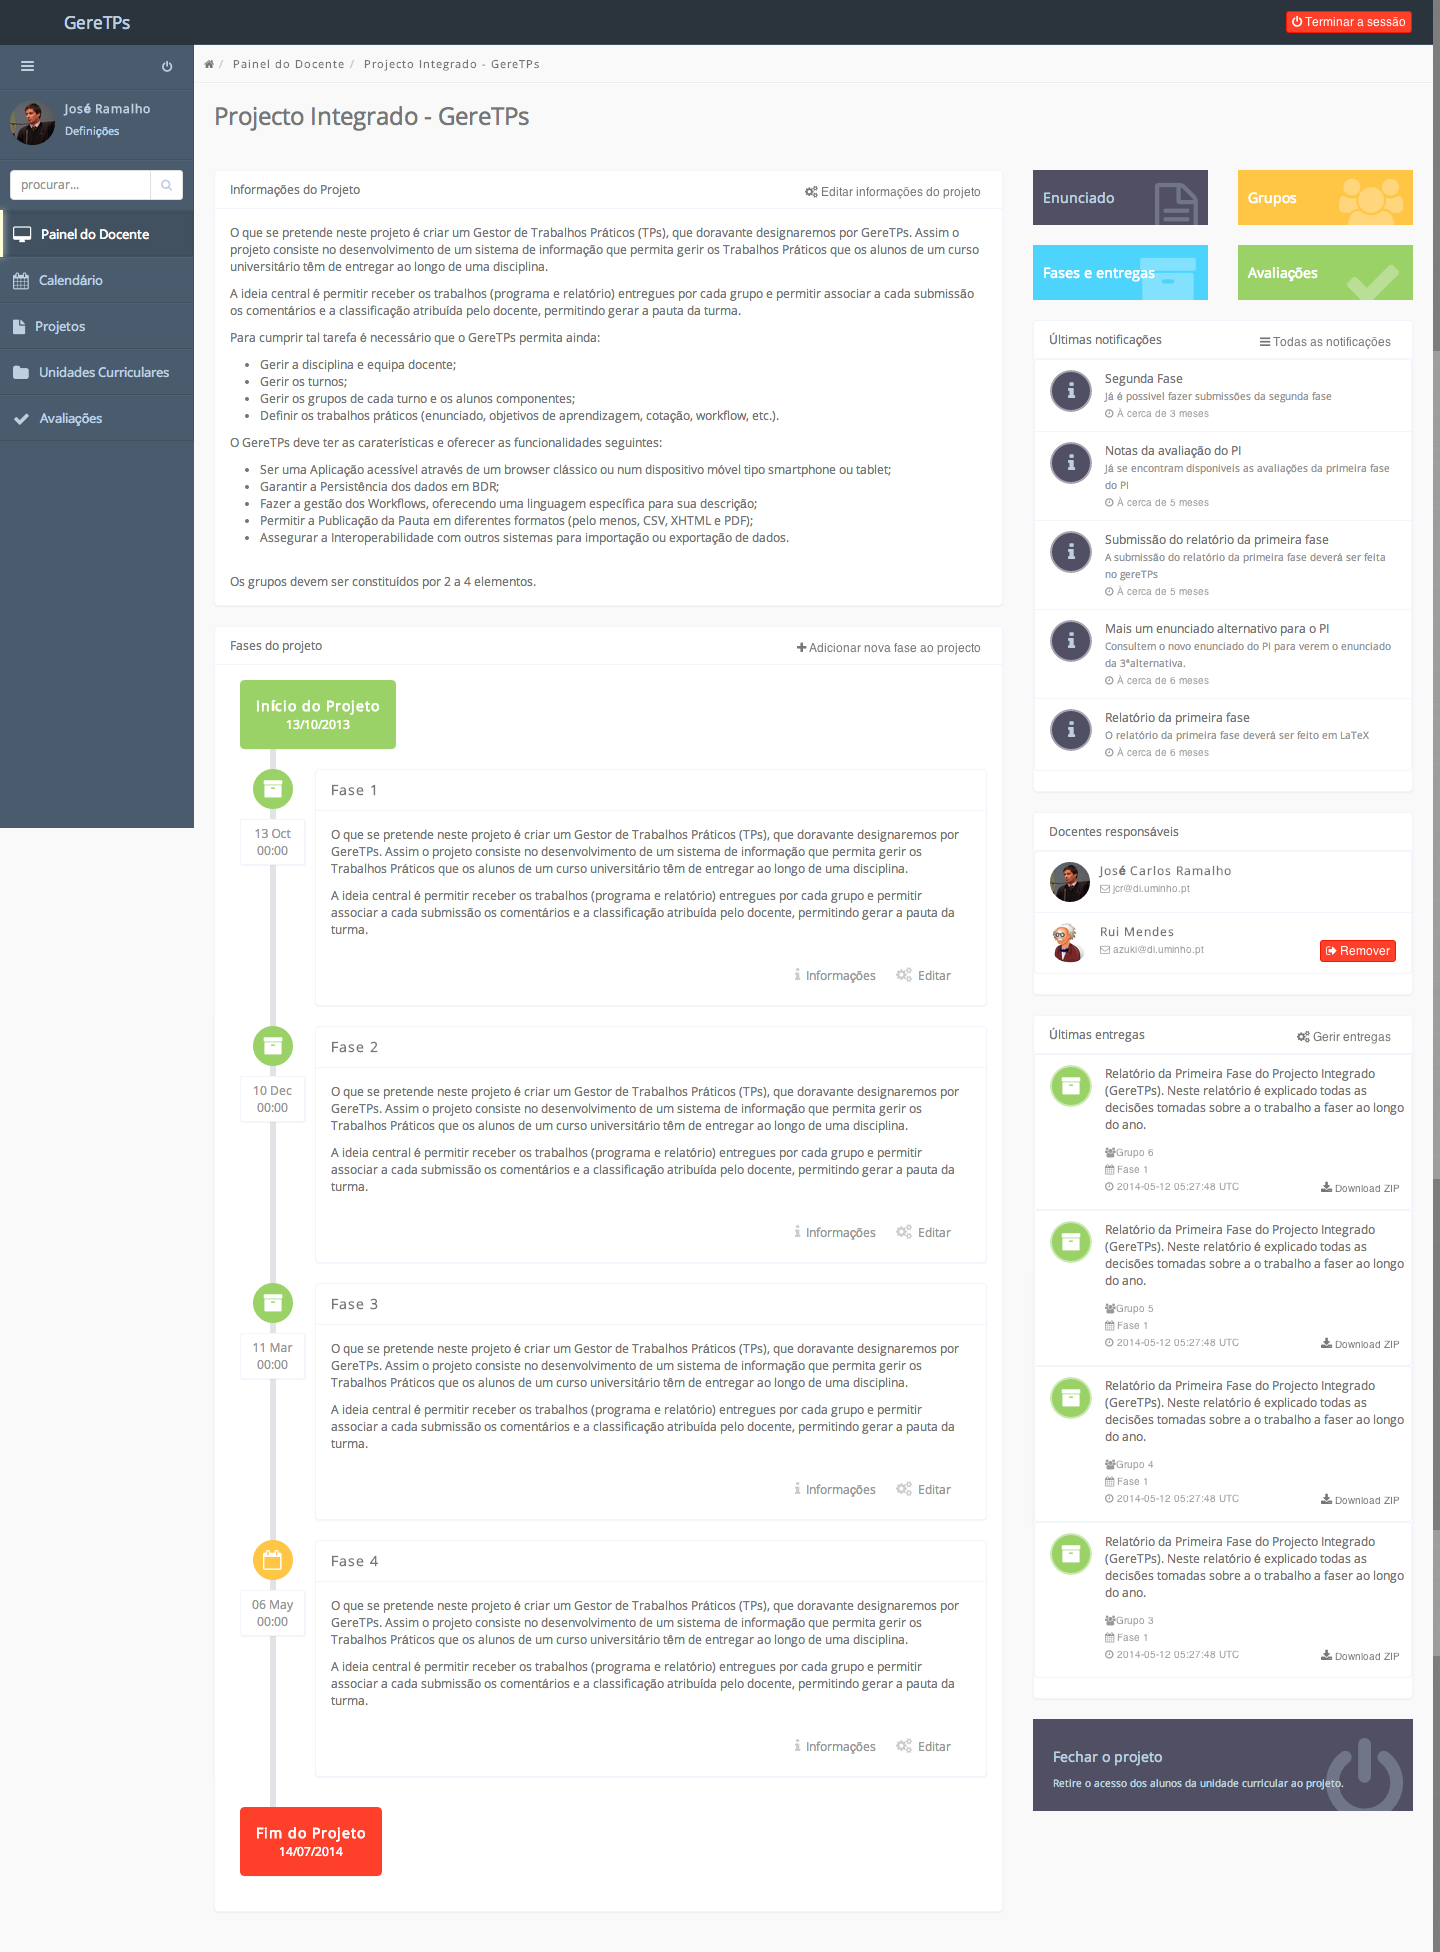
\includegraphics[width=.8\textwidth,center]{images/implementacao/docentes/project}
  \caption{Página de projeto}
  \label{fig:teacher_project}
\end{figure}
